% METADATA SUBSTRATE DESIGN VISUALS V2
% As-built metadata substrate plus proposed persistent-cache/freshness extension.
% Compile: pdflatex METADATA_DESIGN_VISUALS.tex (twice)
\documentclass[10pt]{article}
\usepackage[a4paper,landscape,margin=9mm]{geometry}
\usepackage[utf8]{inputenc}
\usepackage[T1]{fontenc}
\usepackage[sc]{mathpazo}
\usepackage{microtype}
\usepackage{tikz}
\usetikzlibrary{arrows.meta,positioning,fit,calc,backgrounds,shapes.geometric,shapes.multipart,matrix}
\usepackage{xcolor}
\usepackage{array,tabularx,booktabs}
\usepackage{adjustbox}
\usepackage{hyperref}
\hypersetup{hidelinks}
\pagestyle{empty}
\setlength{\parindent}{0pt}
\setlength{\tabcolsep}{4pt}
\renewcommand{\arraystretch}{1.16}

% Palette: same family as the STS2 review diagrams, tuned for print.
\definecolor{store}{HTML}{EAF0FF}
\definecolor{snap}{HTML}{EAF8EC}
\definecolor{engine}{HTML}{FFF3E4}
\definecolor{session}{HTML}{FFF0EE}
\definecolor{gate}{HTML}{E8F7F5}
\definecolor{obs}{HTML}{F6EDFA}
\definecolor{future}{HTML}{FFF9D9}
\definecolor{risk}{HTML}{FFE3E3}
\definecolor{good}{HTML}{E2F5E7}
\definecolor{external}{HTML}{F5F5F5}
\definecolor{ink}{HTML}{263238}
\definecolor{muted}{HTML}{607D8B}
\definecolor{green}{HTML}{39784A}
\definecolor{orange}{HTML}{B56A24}
\definecolor{red}{HTML}{B54A4A}
\definecolor{blue}{HTML}{3F6FB5}
\definecolor{purple}{HTML}{7A4E9B}

\newcommand{\code}[1]{\texttt{\detokenize{#1}}}
\newcommand{\yes}{\textbf{yes}}
\newcommand{\no}{\textbf{no}}
\newcommand{\maybe}{\textbf{maybe}}

\tikzset{
  >=Latex,
  every node/.style={font=\small,text=ink},
  box/.style={draw=ink!55,rounded corners=2.5pt,fill=store,align=center,inner sep=4pt,minimum height=10mm},
  snapbox/.style={box,fill=snap,draw=green!65},
  enginebox/.style={box,fill=engine,draw=orange!70},
  sessbox/.style={box,fill=session,draw=red!65},
  gatebox/.style={box,fill=gate,draw=green!70},
  obsbox/.style={box,fill=obs,draw=purple!65},
  futurebox/.style={box,fill=future,draw=orange!80},
  riskbox/.style={box,fill=risk,draw=red!75},
  goodbox/.style={box,fill=good,draw=green!75},
  extbox/.style={box,fill=external,draw=ink!45,dashed},
  state/.style={draw=ink!60,rounded corners=7pt,fill=store,minimum width=29mm,minimum height=10mm,align=center,inner sep=3pt},
  arrow/.style={->,very thick,draw=ink!75},
  thinarr/.style={->,thick,draw=ink!65},
  dashedarr/.style={->,thick,dashed,draw=purple!80},
  hot/.style={->,very thick,draw=red!80},
  note/.style={draw=ink!25,rounded corners=2pt,fill=white,align=left,inner sep=5pt,font=\footnotesize,text width=62mm},
  smallnote/.style={draw=ink!25,rounded corners=2pt,fill=white,align=left,inner sep=4pt,font=\scriptsize,text width=42mm},
  pill/.style={draw=ink!35,rounded corners=7pt,fill=white,inner xsep=5pt,inner ysep=2pt,font=\footnotesize\bfseries},
  caption/.style={font=\scriptsize,align=center,fill=white,inner sep=1.3pt},
}

\newcommand{\pagehead}[2]{%
  \begin{minipage}[t]{0.72\linewidth}
    {\Large\bfseries #1}\\[-1mm]
    {\small\color{muted}#2}
  \end{minipage}\hfill
  \begin{minipage}[t]{0.26\linewidth}\raggedleft
    {\footnotesize Metadata substrate - review visuals v2}\\
    {\scriptsize vscode-mssql dev/query checked 2026-07-06}
  \end{minipage}
  \vspace{2.5mm}\hrule\vspace{3.5mm}
}

\newcommand{\legend}{%
\tikz[baseline=-0.7ex]\node[box,minimum width=7mm,minimum height=4mm,inner sep=1pt]{}; store/registry\quad
\tikz[baseline=-0.7ex]\node[snapbox,minimum width=7mm,minimum height=4mm,inner sep=1pt]{}; pure snapshot\quad
\tikz[baseline=-0.7ex]\node[enginebox,minimum width=7mm,minimum height=4mm,inner sep=1pt]{}; engine/hydration\quad
\tikz[baseline=-0.7ex]\node[sessbox,minimum width=7mm,minimum height=4mm,inner sep=1pt]{}; sessions/data plane\quad
\tikz[baseline=-0.7ex]\node[gatebox,minimum width=7mm,minimum height=4mm,inner sep=1pt]{}; contract/privacy gate\quad
\tikz[baseline=-0.7ex]\node[futurebox,minimum width=7mm,minimum height=4mm,inner sep=1pt]{}; proposed cache\quad
\tikz[baseline=-0.7ex]\node[obsbox,minimum width=7mm,minimum height=4mm,inner sep=1pt]{}; observability
}

\begin{document}

% =====================================================================
% 1. SUBSTRATE MAP
% =====================================================================
\pagehead{1. Metadata substrate at a glance}
{The substrate is strongest where it is boring: two seams above one store, immutable views below, and no consumer gets to improvise catalog truth.}
\legend\par\vspace{4mm}

\begin{adjustbox}{max width=\linewidth,max height=0.82\textheight,center}
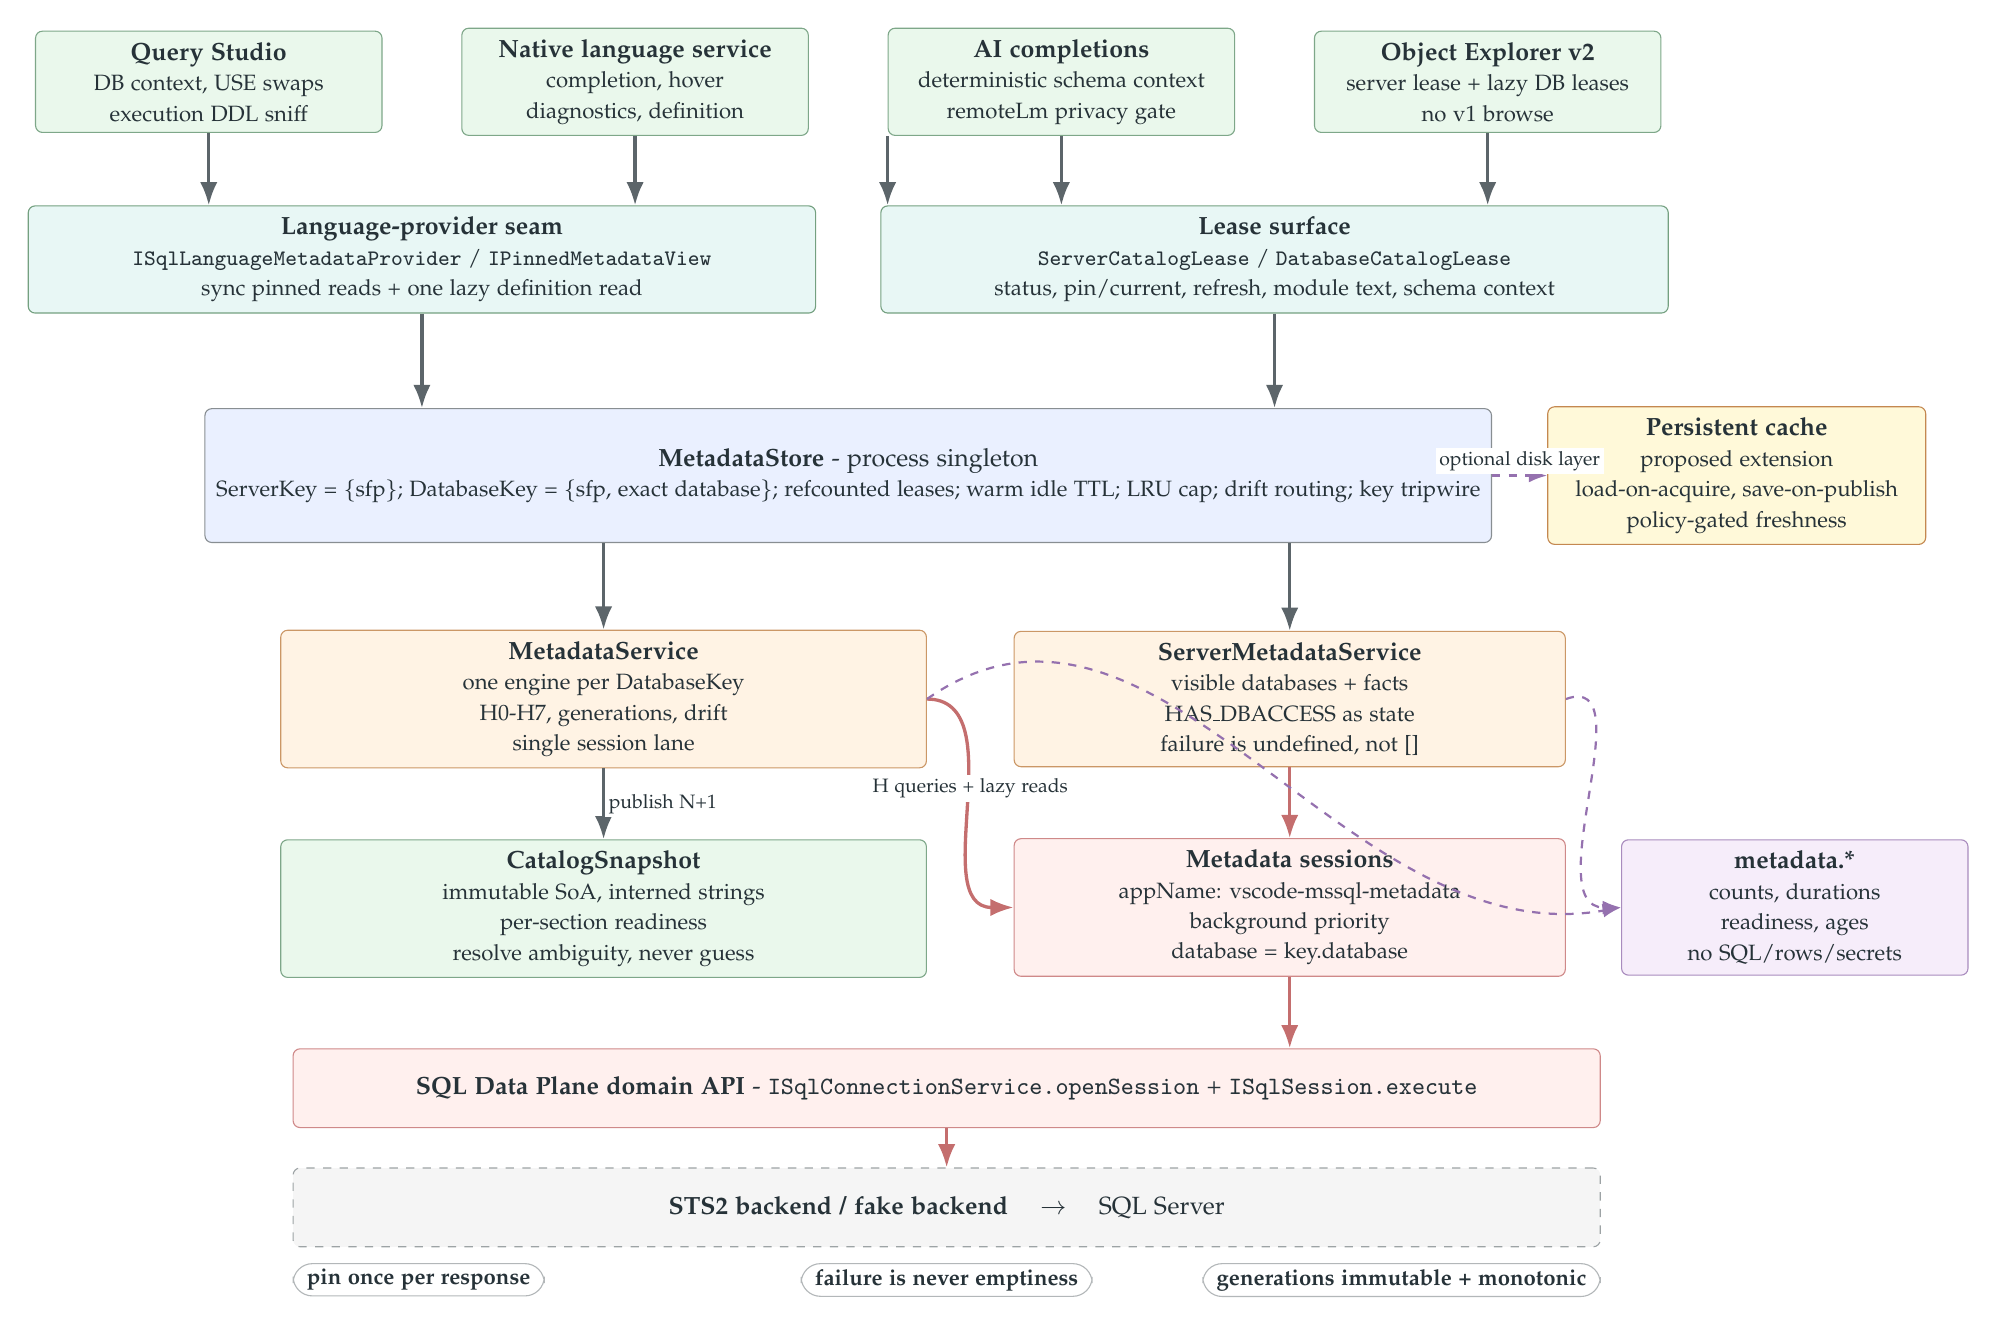
\begin{tikzpicture}[node distance=7mm and 10mm]

% Consumers
\node[snapbox,minimum width=44mm] (qs) {\textbf{Query Studio}\\\footnotesize DB context, USE swaps\\\footnotesize execution DDL sniff};
\node[snapbox,minimum width=44mm,right=of qs] (ls) {\textbf{Native language service}\\\footnotesize completion, hover\\\footnotesize diagnostics, definition};
\node[snapbox,minimum width=44mm,right=of ls] (ai) {\textbf{AI completions}\\\footnotesize deterministic schema context\\\footnotesize remoteLm privacy gate};
\node[snapbox,minimum width=44mm,right=of ai] (oe) {\textbf{Object Explorer v2}\\\footnotesize server lease + lazy DB leases\\\footnotesize no v1 browse};

% Seams
\node[gatebox,minimum width=100mm,below=9mm of $(qs.south)!0.5!(ls.south)$] (langseam) {\textbf{Language-provider seam}\\\footnotesize \code{ISqlLanguageMetadataProvider} / \code{IPinnedMetadataView}\\\footnotesize sync pinned reads + one lazy definition read};
\node[gatebox,minimum width=100mm,below=9mm of $(ai.south)!0.5!(oe.south)$] (leases) {\textbf{Lease surface}\\\footnotesize \code{ServerCatalogLease} / \code{DatabaseCatalogLease}\\\footnotesize status, pin/current, refresh, module text, schema context};

% Store and cache extension
\node[box,minimum width=154mm,minimum height=17mm,below=12mm of $(langseam.south)!0.5!(leases.south)$] (store) {\textbf{MetadataStore} - process singleton\\\footnotesize ServerKey = \{sfp\}; DatabaseKey = \{sfp, exact database\}; refcounted leases; warm idle TTL; LRU cap; drift routing; key tripwire};
\node[futurebox,minimum width=48mm,minimum height=17mm,right=7mm of store] (pcache) {\textbf{Persistent cache}\\\footnotesize proposed extension\\\footnotesize load-on-acquire, save-on-publish\\\footnotesize policy-gated freshness};

% Engines and snapshot
\node[enginebox,minimum width=82mm,below left=11mm and -10mm of store.south] (dbengine) {\textbf{MetadataService}\\\footnotesize one engine per DatabaseKey\\\footnotesize H0-H7, generations, drift\\\footnotesize single session lane};
\node[enginebox,minimum width=70mm,right=11mm of dbengine] (serverengine) {\textbf{ServerMetadataService}\\\footnotesize visible databases + facts\\\footnotesize HAS\_DBACCESS as state\\\footnotesize failure is undefined, not []};
\node[snapbox,minimum width=82mm,below=9mm of dbengine] (snapshot) {\textbf{CatalogSnapshot}\\\footnotesize immutable SoA, interned strings\\\footnotesize per-section readiness\\\footnotesize resolve ambiguity, never guess};
\node[sessbox,minimum width=70mm,below=9mm of serverengine] (sessions) {\textbf{Metadata sessions}\\\footnotesize appName: vscode-mssql-metadata\\\footnotesize background priority\\\footnotesize database = key.database};
\node[sessbox,minimum width=166mm,below=9mm of $(snapshot.south)!0.5!(sessions.south)$] (dp) {\textbf{SQL Data Plane domain API} - \code{ISqlConnectionService.openSession} + \code{ISqlSession.execute}};
\node[extbox,minimum width=166mm,below=5mm of dp] (sql) {\textbf{STS2 backend / fake backend} \quad $\to$ \quad SQL Server};

% Observability
\node[obsbox,minimum width=44mm,right=7mm of sessions] (obs) {\textbf{metadata.*}\\\footnotesize counts, durations\\\footnotesize readiness, ages\\\footnotesize no SQL/rows/secrets};

% Arrows
\foreach \c in {qs,ls} {\draw[arrow] (\c.south) -- (langseam.north -| \c.south);}
\draw[arrow] (ai.south west) -- (langseam.north -| ai.south west);
\draw[arrow] (ai.south) -- (leases.north -| ai.south);
\draw[arrow] (oe.south) -- (leases.north -| oe.south);
\draw[arrow] (langseam.south) -- (store.north -| langseam.south);
\draw[arrow] (leases.south) -- (store.north -| leases.south);
\draw[dashedarr] (store.east) -- node[caption,above]{optional disk layer} (pcache.west);
\draw[arrow] (store.south -| dbengine.north) -- (dbengine.north);
\draw[arrow] (store.south -| serverengine.north) -- (serverengine.north);
\draw[arrow] (dbengine.south) -- node[caption,right]{publish N+1} (snapshot.north);
\draw[hot] (dbengine.east) to[out=0,in=180] node[caption,above]{H queries + lazy reads} (sessions.west);
\draw[hot] (serverengine.south) -- (sessions.north);
\draw[hot] (sessions.south) -- (dp.north -| sessions.south);
\draw[hot] (dp.south) -- (sql.north);
\draw[dashedarr] (dbengine.east) to[out=35,in=190] (obs.west);
\draw[dashedarr] (serverengine.east) to[out=20,in=180] (obs.west);

\node[pill,below=2mm of sql.south west,anchor=north west] {pin once per response};
\node[pill,below=2mm of sql.south,anchor=north] {failure is never emptiness};
\node[pill,below=2mm of sql.south east,anchor=north east] {generations immutable + monotonic};

\end{tikzpicture}
\end{adjustbox}

\newpage

% =====================================================================
% 2. KEYS AND LEASES
% =====================================================================
\pagehead{2. Identity, key-correctness, and leases}
{Database isolation is enforced by construction first, then watched by a tripwire. Warm memory reuse is separate from the proposed persistent cache.}
\legend\par\vspace{4mm}

\begin{adjustbox}{max width=\linewidth,max height=0.82\textheight,center}
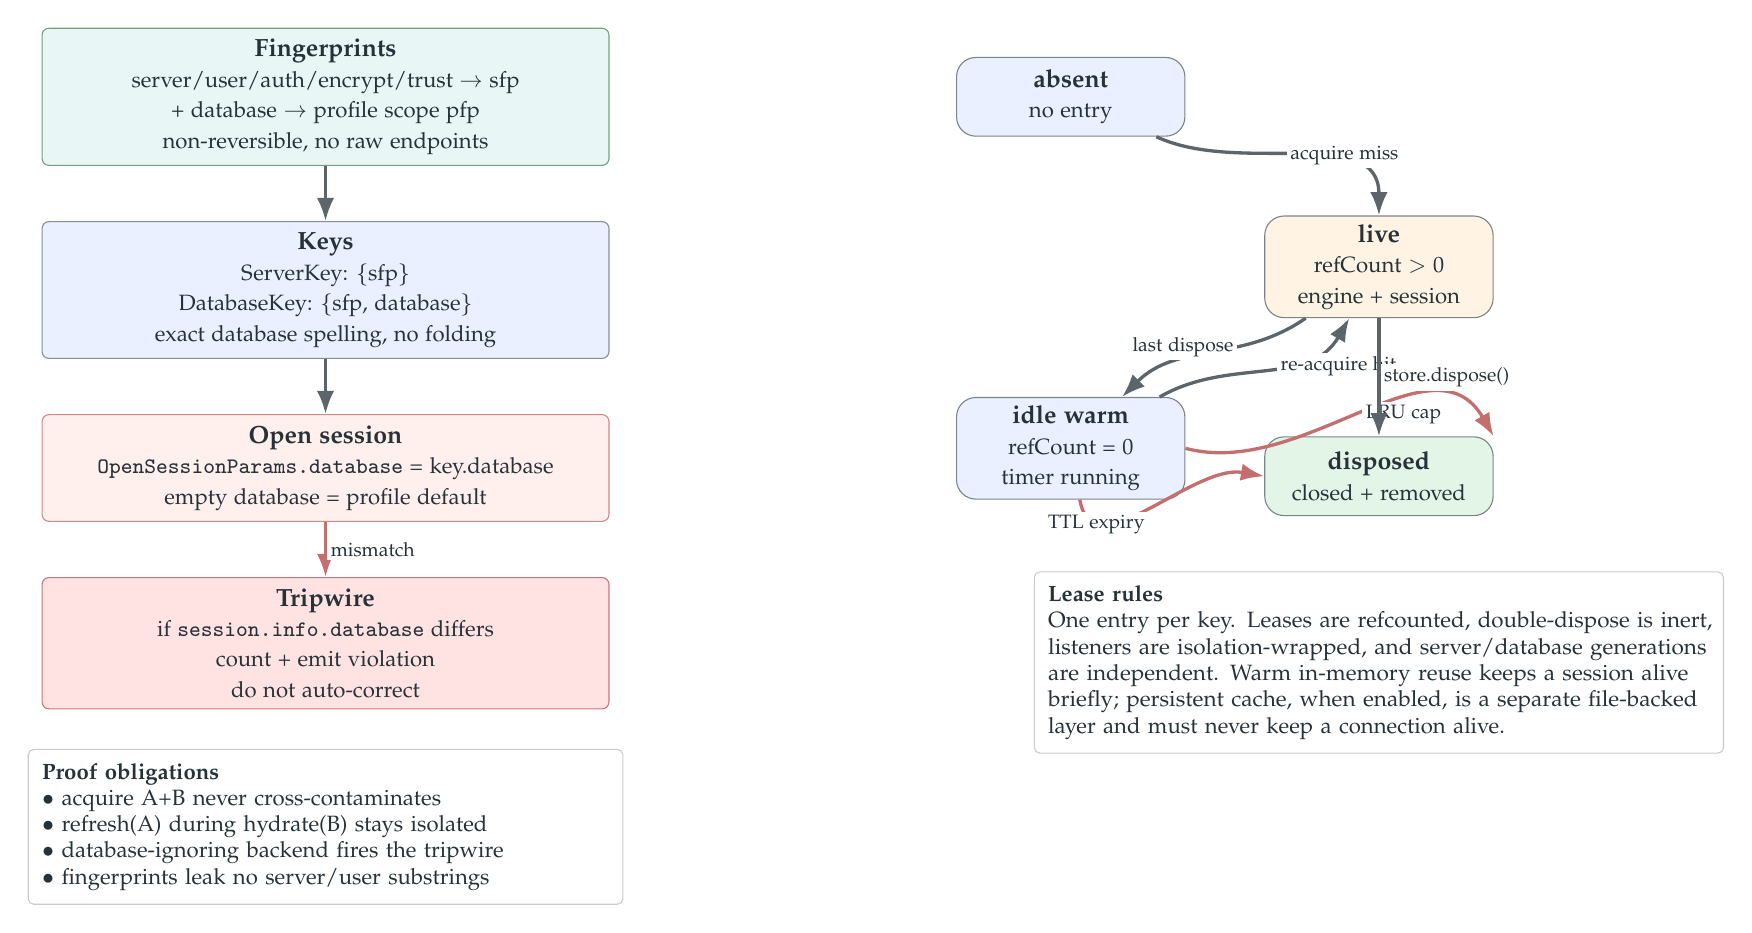
\begin{tikzpicture}[node distance=7mm and 9mm]

\node[gatebox,minimum width=72mm] (fingerprints) {\textbf{Fingerprints}\\\footnotesize server/user/auth/encrypt/trust $\to$ sfp\\\footnotesize + database $\to$ profile scope pfp\\\footnotesize non-reversible, no raw endpoints};
\node[box,minimum width=72mm,below=of fingerprints] (keys) {\textbf{Keys}\\\footnotesize ServerKey: \{sfp\}\\\footnotesize DatabaseKey: \{sfp, database\}\\\footnotesize exact database spelling, no folding};
\node[sessbox,minimum width=72mm,below=of keys] (opens) {\textbf{Open session}\\\footnotesize \code{OpenSessionParams.database} = key.database\\\footnotesize empty database = profile default};
\node[riskbox,minimum width=72mm,below=of opens] (tripwire) {\textbf{Tripwire}\\\footnotesize if \code{session.info.database} differs\\\footnotesize count + emit violation\\\footnotesize do not auto-correct};
\draw[arrow] (fingerprints) -- (keys);
\draw[arrow] (keys) -- (opens);
\draw[hot] (opens) -- node[caption,right]{mismatch} (tripwire);

\node[state,right=44mm of fingerprints] (absent) {\textbf{absent}\\\footnotesize no entry};
\node[state,fill=engine,below right=10mm and 10mm of absent] (live) {\textbf{live}\\\footnotesize refCount $>$ 0\\\footnotesize engine + session};
\node[state,below left=10mm and 10mm of live] (idle) {\textbf{idle warm}\\\footnotesize refCount = 0\\\footnotesize timer running};
\node[state,fill=good,below=15mm of live] (disposed) {\textbf{disposed}\\\footnotesize closed + removed};

\draw[arrow] (absent) to[out=-25,in=90] node[caption,right,pos=0.45]{acquire miss} (live);
\draw[arrow] (live) to[out=-145,in=45] node[caption,left,pos=0.35]{last dispose} (idle);
\draw[arrow] (idle) to[out=30,in=-120] node[caption,right,pos=0.55]{re-acquire hit} (live);
\draw[hot] (idle) to[out=-80,in=170] node[caption,below left]{TTL expiry} (disposed.west);
\draw[hot] (idle.east) to[out=-15,in=120] node[caption,right]{LRU cap} (disposed.north east);
\draw[arrow] (live) -- node[caption,right]{store.dispose()} (disposed);

\node[note,below=5mm of tripwire,text width=72mm] (proofs) {\textbf{Proof obligations}\\
$\bullet$ acquire A+B never cross-contaminates\\
$\bullet$ refresh(A) during hydrate(B) stays isolated\\
$\bullet$ database-ignoring backend fires the tripwire\\
$\bullet$ fingerprints leak no server/user substrings};

\node[note,below=7mm of disposed,text width=84mm] (lease) {\textbf{Lease rules}\\
One entry per key. Leases are refcounted, double-dispose is inert, listeners are isolation-wrapped, and server/database generations are independent. Warm in-memory reuse keeps a session alive briefly; persistent cache, when enabled, is a separate file-backed layer and must never keep a connection alive.};

\end{tikzpicture}
\end{adjustbox}

\newpage

% =====================================================================
% 3. HYDRATION
% =====================================================================
\pagehead{3. Hydration ladder and readiness honesty}
{The ladder deepens in strict order, but later sections fail independently. Consumers must read section state before trusting an empty result.}
\legend\par\vspace{4mm}

\begin{adjustbox}{max width=\linewidth,max height=0.82\textheight,center}
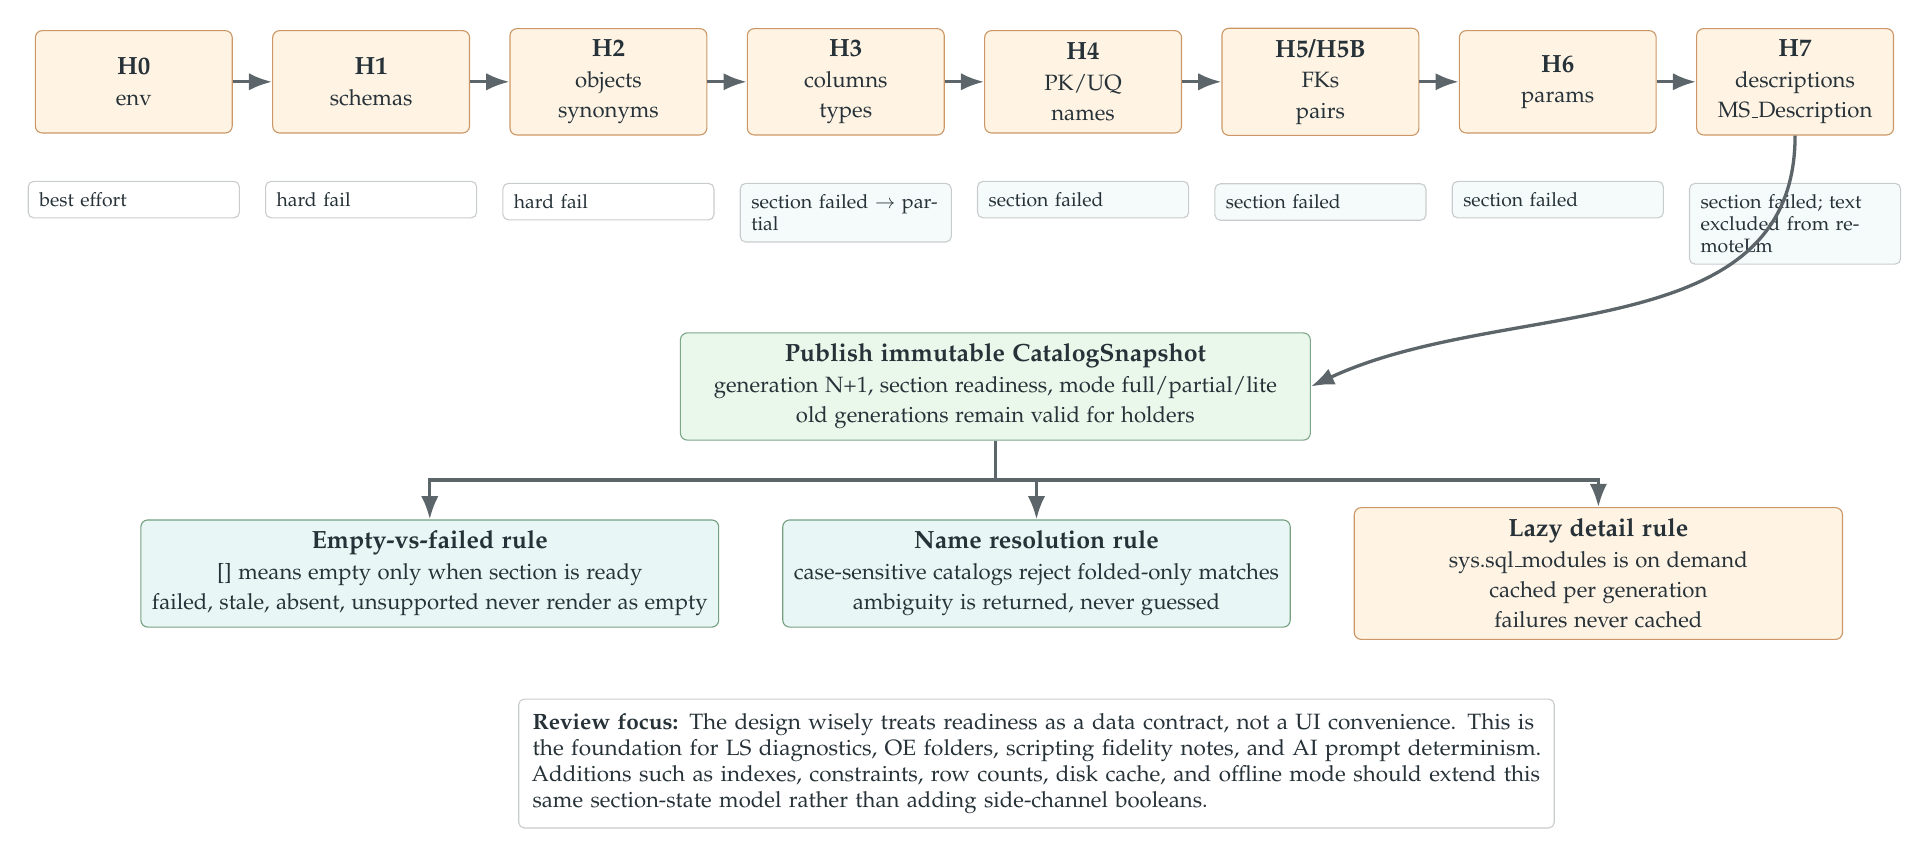
\begin{tikzpicture}[node distance=4mm and 5mm]

\node[enginebox,minimum width=25mm,minimum height=13mm] (h0) {\textbf{H0}\\\footnotesize env};
\node[enginebox,minimum width=25mm,minimum height=13mm,right=of h0] (h1) {\textbf{H1}\\\footnotesize schemas};
\node[enginebox,minimum width=25mm,minimum height=13mm,right=of h1] (h2) {\textbf{H2}\\\footnotesize objects\\\footnotesize synonyms};
\node[enginebox,minimum width=25mm,minimum height=13mm,right=of h2] (h3) {\textbf{H3}\\\footnotesize columns\\\footnotesize types};
\node[enginebox,minimum width=25mm,minimum height=13mm,right=of h3] (h4) {\textbf{H4}\\\footnotesize PK/UQ\\\footnotesize names};
\node[enginebox,minimum width=25mm,minimum height=13mm,right=of h4] (h5) {\textbf{H5/H5B}\\\footnotesize FKs\\\footnotesize pairs};
\node[enginebox,minimum width=25mm,minimum height=13mm,right=of h5] (h6) {\textbf{H6}\\\footnotesize params};
\node[enginebox,minimum width=25mm,minimum height=13mm,right=of h6] (h7) {\textbf{H7}\\\footnotesize descriptions\\\footnotesize MS\_Description};
\foreach \a/\b in {h0/h1,h1/h2,h2/h3,h3/h4,h4/h5,h5/h6,h6/h7}{\draw[arrow] (\a.east) -- (\b.west);}

\node[smallnote,below=6mm of h0,text width=24mm] {best effort};
\node[smallnote,below=6mm of h1,text width=24mm] {hard fail};
\node[smallnote,below=6mm of h2,text width=24mm] {hard fail};
\node[smallnote,below=6mm of h3,text width=24mm,fill=gate!45] {section failed $\to$ partial};
\node[smallnote,below=6mm of h4,text width=24mm,fill=gate!45] {section failed};
\node[smallnote,below=6mm of h5,text width=24mm,fill=gate!45] {section failed};
\node[smallnote,below=6mm of h6,text width=24mm,fill=gate!45] {section failed};
\node[smallnote,below=6mm of h7,text width=24mm,fill=gate!45] {section failed; text excluded from remoteLm};

\node[snapbox,minimum width=80mm,below=25mm of h3.south,xshift=19mm] (publish) {\textbf{Publish immutable CatalogSnapshot}\\\footnotesize generation N+1, section readiness, mode full/partial/lite\\\footnotesize old generations remain valid for holders};
\draw[arrow] (h7.south) to[out=-90,in=25] (publish.east);

\node[gatebox,minimum width=62mm,below left=10mm and -5mm of publish] (empty) {\textbf{Empty-vs-failed rule}\\\footnotesize [] means empty only when section is ready\\\footnotesize failed, stale, absent, unsupported never render as empty};
\node[gatebox,minimum width=62mm,right=8mm of empty] (resolve) {\textbf{Name resolution rule}\\\footnotesize case-sensitive catalogs reject folded-only matches\\\footnotesize ambiguity is returned, never guessed};
\node[enginebox,minimum width=62mm,right=8mm of resolve] (lazy) {\textbf{Lazy detail rule}\\\footnotesize sys.sql\_modules is on demand\\\footnotesize cached per generation\\\footnotesize failures never cached};

\draw[arrow] (publish.south) -- ++(0,-5mm) -| (empty.north);
\draw[arrow] (publish.south) -- ++(0,-5mm) -| (resolve.north);
\draw[arrow] (publish.south) -- ++(0,-5mm) -| (lazy.north);

\node[note,below=9mm of resolve,text width=128mm] {\textbf{Review focus:} The design wisely treats readiness as a data contract, not a UI convenience. This is the foundation for LS diagnostics, OE folders, scripting fidelity notes, and AI prompt determinism. Additions such as indexes, constraints, row counts, disk cache, and offline mode should extend this same section-state model rather than adding side-channel booleans.};

\end{tikzpicture}
\end{adjustbox}

\newpage

% =====================================================================
% 4. DRIFT LOOP
% =====================================================================
\pagehead{4. Drift detection and refresh orchestration}
{The current loop is cheap and safe. The cache proposal adds policy-aware validation so strict consumers can demand fresher proof than completion needs.}
\legend\par\vspace{4mm}

\begin{adjustbox}{max width=\linewidth,max height=0.82\textheight,center}
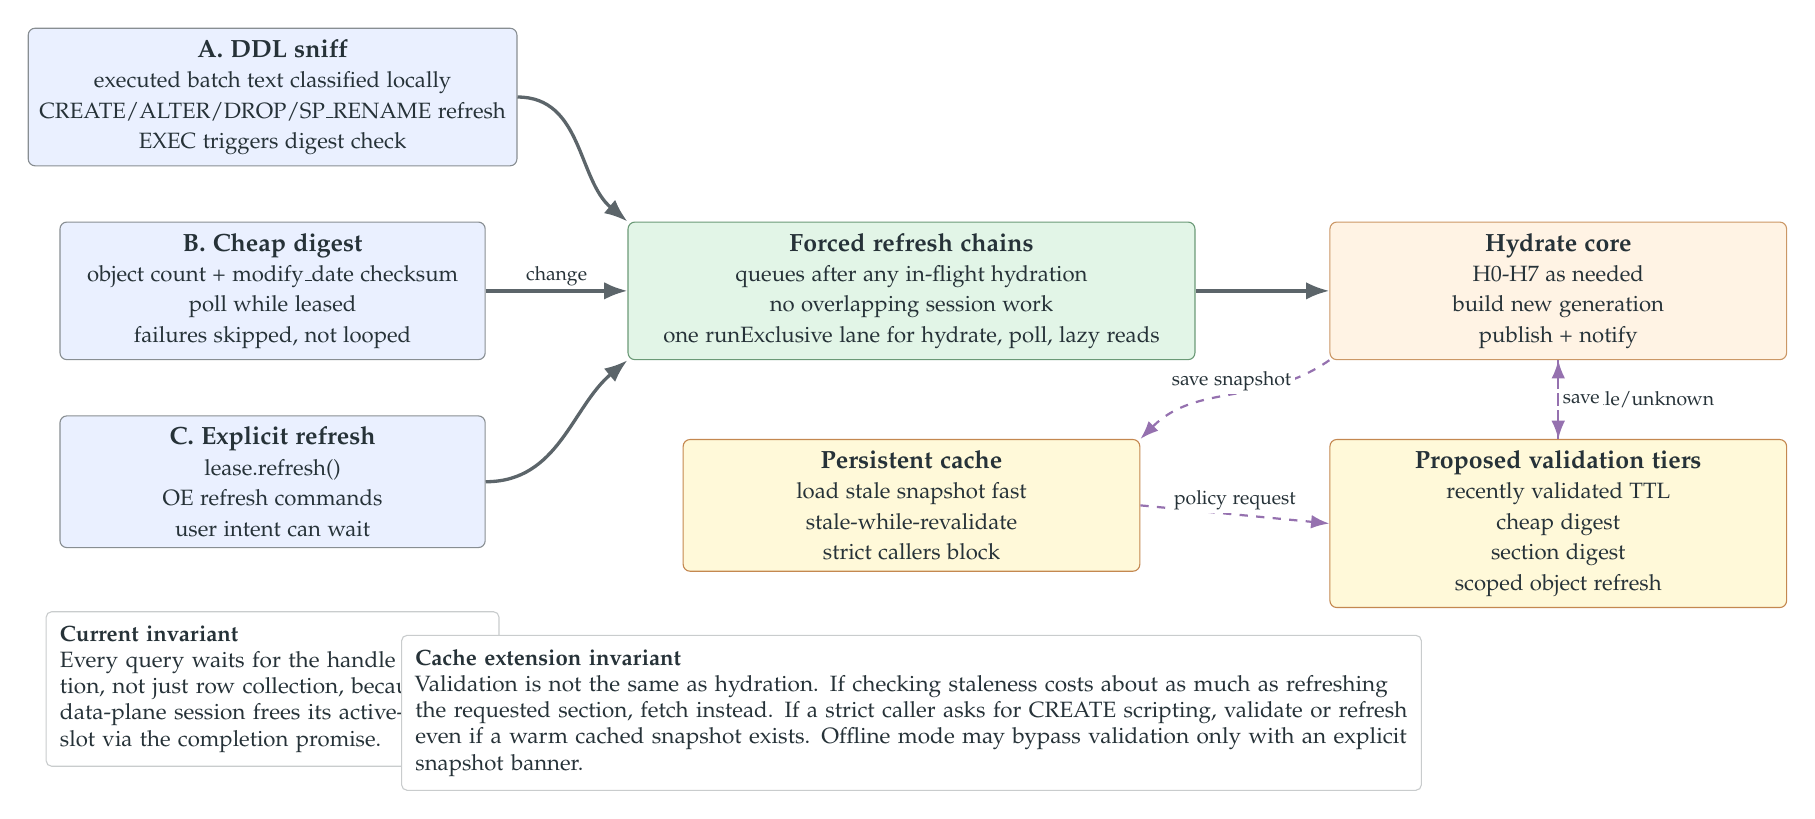
\begin{tikzpicture}[node distance=7mm and 9mm]

\node[box,minimum width=54mm] (sniff) {\textbf{A. DDL sniff}\\\footnotesize executed batch text classified locally\\\footnotesize CREATE/ALTER/DROP/SP\_RENAME refresh\\\footnotesize EXEC triggers digest check};
\node[box,minimum width=54mm,below=of sniff] (digest) {\textbf{B. Cheap digest}\\\footnotesize object count + modify\_date checksum\\\footnotesize poll while leased\\\footnotesize failures skipped, not looped};
\node[box,minimum width=54mm,below=of digest] (explicit) {\textbf{C. Explicit refresh}\\\footnotesize lease.refresh()\\\footnotesize OE refresh commands\\\footnotesize user intent can wait};

\node[goodbox,minimum width=72mm,right=18mm of digest] (chain) {\textbf{Forced refresh chains}\\\footnotesize queues after any in-flight hydration\\\footnotesize no overlapping session work\\\footnotesize one runExclusive lane for hydrate, poll, lazy reads};

\node[enginebox,minimum width=58mm,right=17mm of chain] (hydrate) {\textbf{Hydrate core}\\\footnotesize H0-H7 as needed\\\footnotesize build new generation\\\footnotesize publish + notify};
\node[futurebox,minimum width=58mm,below=10mm of hydrate] (validate) {\textbf{Proposed validation tiers}\\\footnotesize recently validated TTL\\\footnotesize cheap digest\\\footnotesize section digest\\\footnotesize scoped object refresh};
\node[futurebox,minimum width=58mm,below=10mm of chain] (cache) {\textbf{Persistent cache}\\\footnotesize load stale snapshot fast\\\footnotesize stale-while-revalidate\\\footnotesize strict callers block};

\draw[arrow] (sniff.east) to[out=0,in=140] (chain.north west);
\draw[arrow] (digest.east) -- node[caption,above]{change} (chain.west);
\draw[arrow] (explicit.east) to[out=0,in=-140] (chain.south west);
\draw[arrow] (chain.east) -- (hydrate.west);
\draw[dashedarr] (cache.east) -- node[caption,above]{policy request} (validate.west);
\draw[dashedarr] (validate.north) -- node[caption,right]{if stale/unknown} (hydrate.south);
\draw[dashedarr] (hydrate.south) -- node[caption,right]{save} (validate.north);
\draw[dashedarr] (hydrate.south west) to[out=-145,in=45] node[caption,above]{save snapshot} (cache.north east);

\node[note,below=8mm of explicit,text width=54mm] {\textbf{Current invariant}\\ Every query waits for the handle completion, not just row collection, because the data-plane session frees its active-query slot via the completion promise.};
\node[note,below=8mm of cache,text width=126mm] {\textbf{Cache extension invariant}\\ Validation is not the same as hydration. If checking staleness costs about as much as refreshing the requested section, fetch instead. If a strict caller asks for CREATE scripting, validate or refresh even if a warm cached snapshot exists. Offline mode may bypass validation only with an explicit snapshot banner.};

\end{tikzpicture}
\end{adjustbox}

\newpage

% =====================================================================
% 5. FRESHNESS MATRIX
% =====================================================================
\pagehead{5. Consumer freshness policy matrix}
{One metadata store can serve fast, possibly stale suggestions and strict, live scripting only if freshness becomes an explicit request contract.}
\legend\par\vspace{4mm}


\begin{adjustbox}{max width=\linewidth,max height=0.77\textheight,center}
\begin{minipage}{0.98\linewidth}
\scriptsize
\begin{tabularx}{\linewidth}{>{\raggedright\arraybackslash}p{29mm} >{\raggedright\arraybackslash}p{38mm} >{\raggedright\arraybackslash}p{42mm} >{\raggedright\arraybackslash}X}
\toprule
\textbf{Consumer} & \textbf{Default freshness} & \textbf{May use cached data} & \textbf{Must validate or refresh} \\
\midrule
Query Studio & recently validated, background refresh & status badges, readiness display, database dropdown during reconnect & USE-triggered lease swap and DDL notification routing \\
Native completions & allow stale; serve instantly & object names, columns, FK join ranking, system catalog context & none on hot path; mark incomplete when required sections are absent or failed \\
Native diagnostics & validated or suppress/demote & lexical and structural diagnostics; cautious hints & schema errors 207/208/209 need recently validated objects and columns or are suppressed \\
Hover/signature & bounded stale for local facts & types, FK badges, proc params when ready & module definitions, descriptions, and authoritative claims may request validation \\
AI completions & allow stale with deterministic generation marker & schema context, excluding descriptions for remoteLm & privacy gates and prompt byte-identity remain mandatory \\
OE v2 & require recent folder validation, TTL based & folder expand if validated inside TTL; stale-while-revalidate for low-risk browse & first expand beyond TTL, refresh, dropped object path, destructive actions \\
Scripting/definition & require live unless offline snapshot mode & offline script with banner and fidelity notes & CREATE/ALTER script, module text, object detail, destructive command prep \\
\bottomrule
\end{tabularx}

\vspace{4mm}
\begin{center}
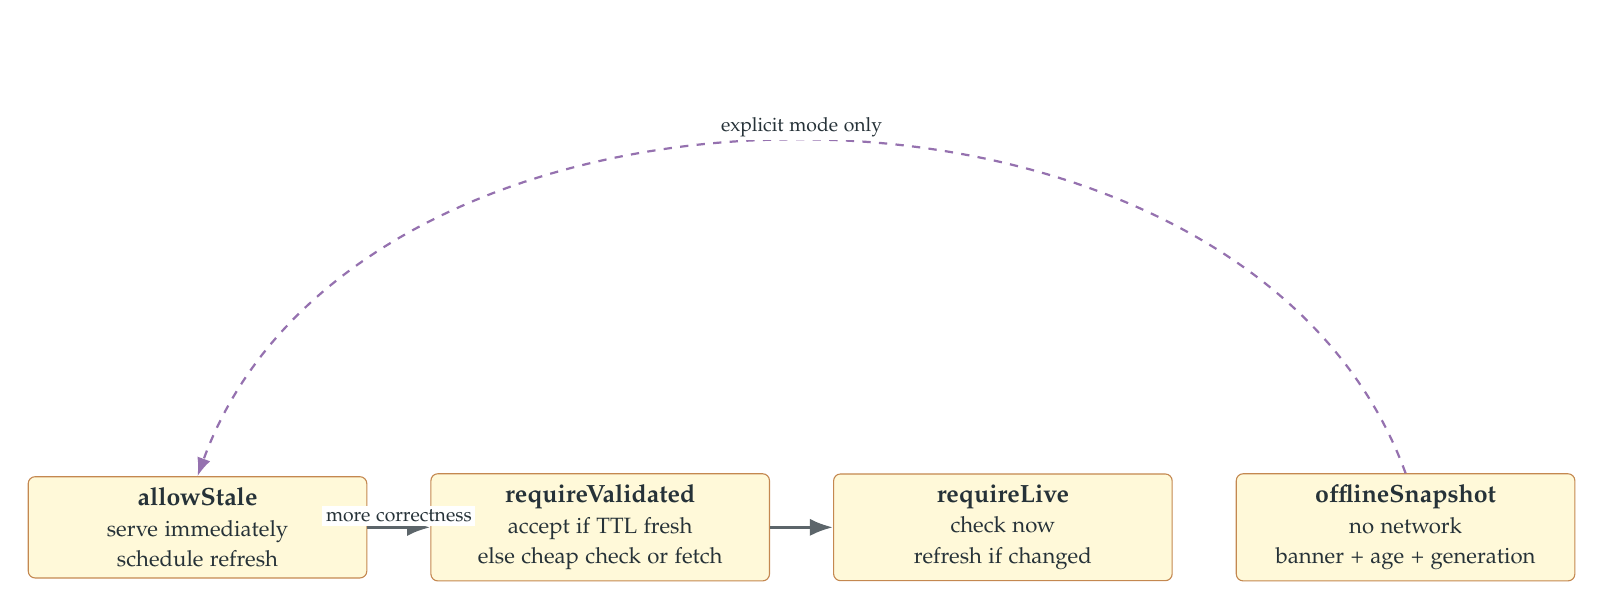
\begin{tikzpicture}[node distance=8mm and 8mm]
\node[futurebox,minimum width=43mm] (stale) {\textbf{allowStale}\\\footnotesize serve immediately\\\footnotesize schedule refresh};
\node[futurebox,minimum width=43mm,right=of stale] (valid) {\textbf{requireValidated}\\\footnotesize accept if TTL fresh\\\footnotesize else cheap check or fetch};
\node[futurebox,minimum width=43mm,right=of valid] (live) {\textbf{requireLive}\\\footnotesize check now\\\footnotesize refresh if changed};
\node[futurebox,minimum width=43mm,right=of live] (offline) {\textbf{offlineSnapshot}\\\footnotesize no network\\\footnotesize banner + age + generation};
\draw[arrow] (stale) -- node[caption,above]{more correctness} (valid);
\draw[arrow] (valid) -- (live);
\draw[dashedarr] (offline.north) to[out=110,in=70] node[caption,above]{explicit mode only} (stale.north);
\end{tikzpicture}
\end{center}

\vspace{2mm}
\begin{center}\footnotesize\textbf{Design rule:} stale data is a performance choice for suggestions, not a license for false diagnostics or wrong scripts.\end{center}
\end{minipage}
\end{adjustbox}

\newpage

% =====================================================================
% 6. PERSISTENT CACHE ARCHITECTURE
% =====================================================================
\pagehead{6. Proposed persistent cache architecture}
{The disk cache is a projection of published snapshots. It loads fast, saves atomically, and never replaces live validation for strict consumers.}
\legend\par\vspace{4mm}

\begin{adjustbox}{max width=\linewidth,max height=0.82\textheight,center}
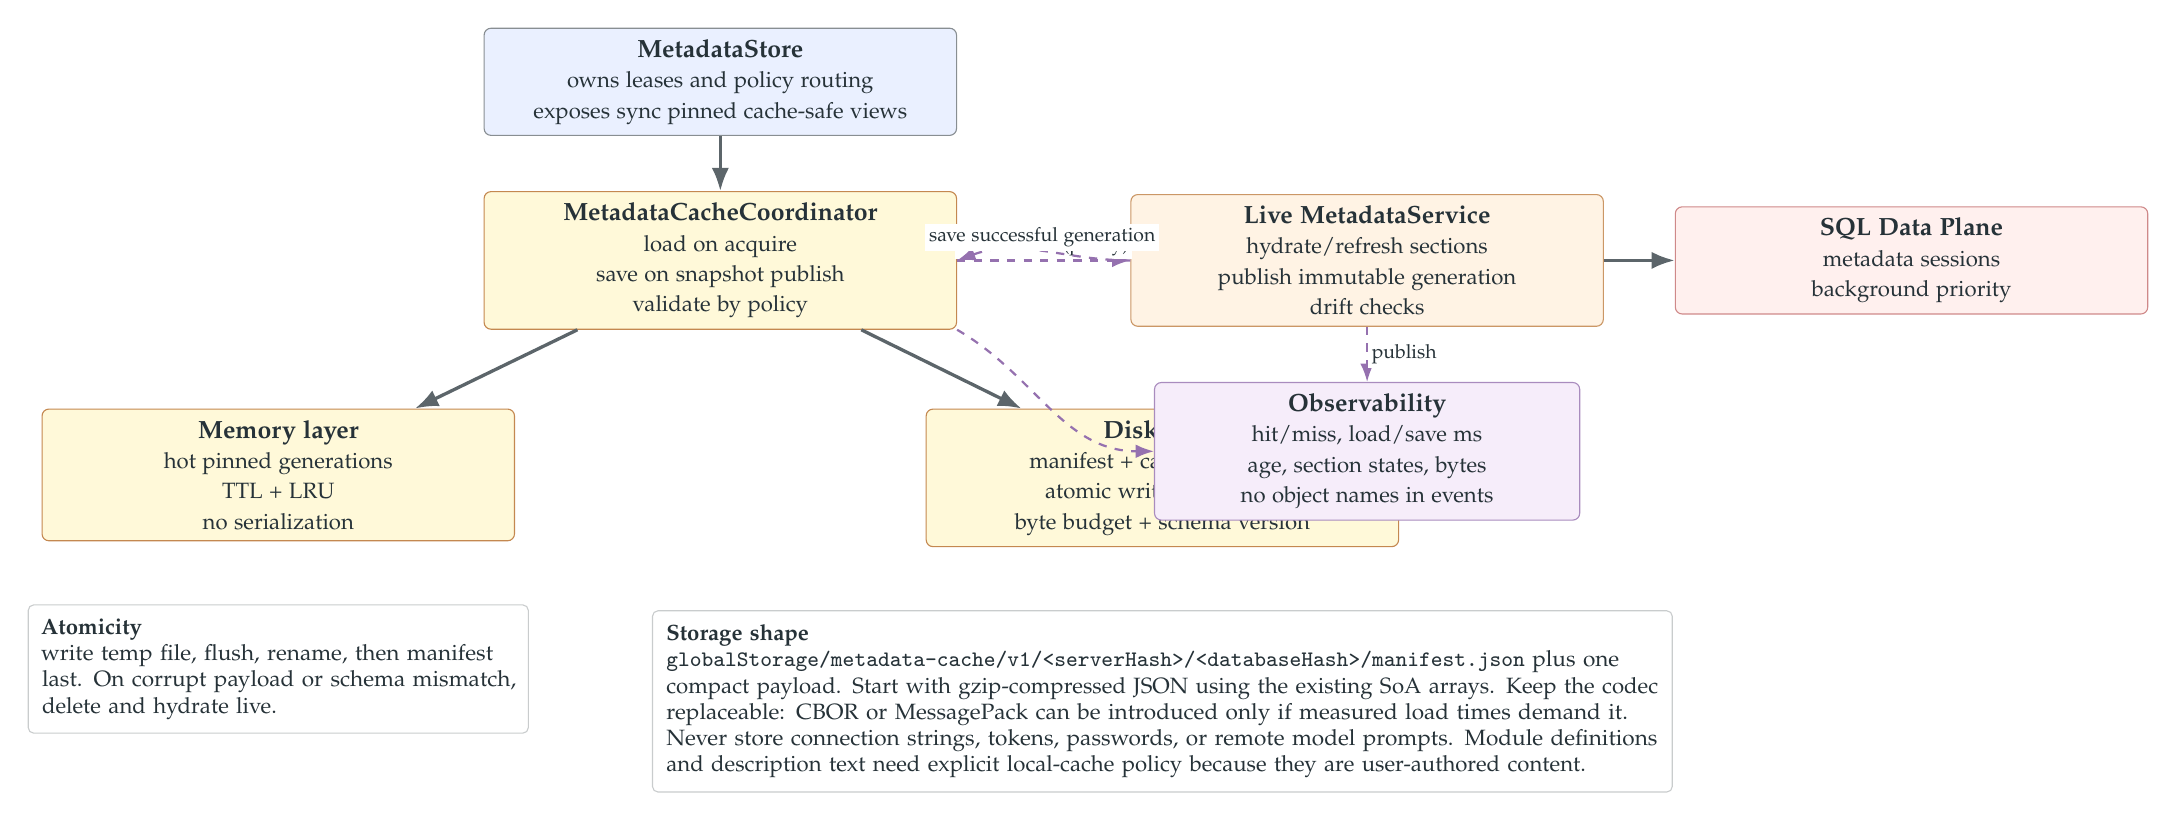
\begin{tikzpicture}[node distance=7mm and 9mm]

\node[box,minimum width=60mm] (store) {\textbf{MetadataStore}\\\footnotesize owns leases and policy routing\\\footnotesize exposes sync pinned cache-safe views};
\node[futurebox,minimum width=60mm,below=of store] (coord) {\textbf{MetadataCacheCoordinator}\\\footnotesize load on acquire\\\footnotesize save on snapshot publish\\\footnotesize validate by policy};
\node[futurebox,minimum width=60mm,below left=10mm and -4mm of coord] (mem) {\textbf{Memory layer}\\\footnotesize hot pinned generations\\\footnotesize TTL + LRU\\\footnotesize no serialization};
\node[futurebox,minimum width=60mm,below right=10mm and -4mm of coord] (disk) {\textbf{Disk layer}\\\footnotesize manifest + catalog payload\\\footnotesize atomic write + recovery\\\footnotesize byte budget + schema version};
\node[enginebox,minimum width=60mm,right=22mm of coord] (live) {\textbf{Live MetadataService}\\\footnotesize hydrate/refresh sections\\\footnotesize publish immutable generation\\\footnotesize drift checks};
\node[sessbox,minimum width=60mm,right=of live] (dp) {\textbf{SQL Data Plane}\\\footnotesize metadata sessions\\\footnotesize background priority};
\node[obsbox,minimum width=54mm,below=of live] (obs) {\textbf{Observability}\\\footnotesize hit/miss, load/save ms\\\footnotesize age, section states, bytes\\\footnotesize no object names in events};

\draw[arrow] (store) -- (coord);
\draw[arrow] (coord) -- (mem);
\draw[arrow] (coord) -- (disk);
\draw[dashedarr] (coord.east) -- node[caption,above]{ensureFresh(policy)} (live.west);
\draw[arrow] (live.east) -- (dp.west);
\draw[dashedarr] (live.south) -- node[caption,right]{publish} (obs.north);
\draw[dashedarr] (coord.south east) to[out=-30,in=180] (obs.west);
\draw[dashedarr] (live.west) to[out=180,in=20] node[caption,above]{save successful generation} (coord.east);

\node[note,below=8mm of disk,text width=126mm] {\textbf{Storage shape}\\
\code{globalStorage/metadata-cache/v1/<serverHash>/<databaseHash>/manifest.json} plus one compact payload. Start with gzip-compressed JSON using the existing SoA arrays. Keep the codec replaceable: CBOR or MessagePack can be introduced only if measured load times demand it. Never store connection strings, tokens, passwords, or remote model prompts. Module definitions and description text need explicit local-cache policy because they are user-authored content.};

\node[note,below=8mm of mem,text width=60mm] {\textbf{Atomicity}\\ write temp file, flush, rename, then manifest last. On corrupt payload or schema mismatch, delete and hydrate live.};

\end{tikzpicture}
\end{adjustbox}

\newpage

% =====================================================================
% 7. CONSUMER FLOWS
% =====================================================================
\pagehead{7. Consumer contracts and privacy gates}
{The same data can feed four very different surfaces only because each surface has a narrow contract and a privacy fence.}
\legend\par\vspace{4mm}

\begin{adjustbox}{max width=\linewidth,max height=0.82\textheight,center}
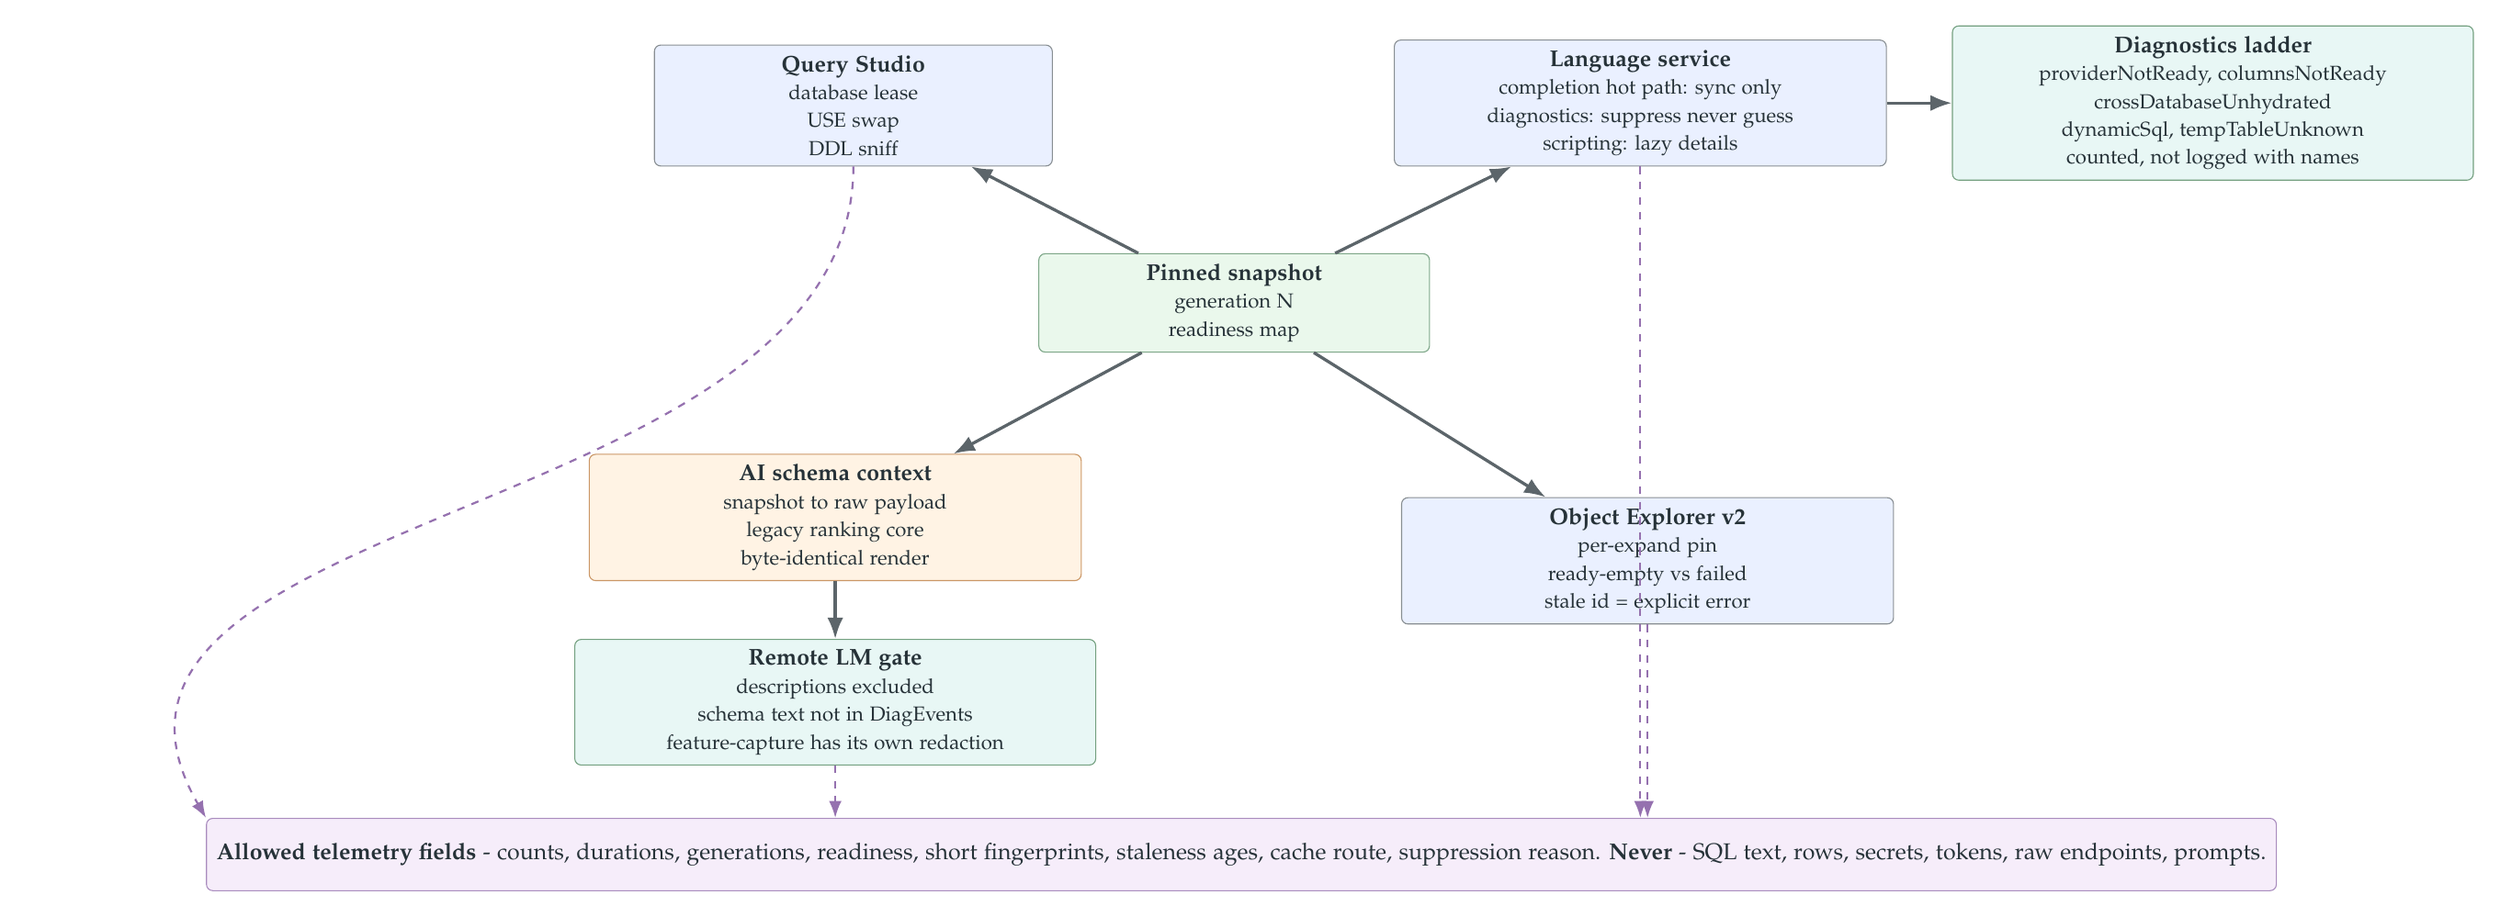
\begin{tikzpicture}[node distance=7mm and 9mm]
\node[snapbox,minimum width=54mm] (snap) {\textbf{Pinned snapshot}\\\footnotesize generation N\\\footnotesize readiness map};

\node[box,minimum width=55mm,above left=12mm and -2mm of snap] (qs) {\textbf{Query Studio}\\\footnotesize database lease\\\footnotesize USE swap\\\footnotesize DDL sniff};
\node[box,minimum width=68mm,above right=12mm and -5mm of snap] (ls) {\textbf{Language service}\\\footnotesize completion hot path: sync only\\\footnotesize diagnostics: suppress never guess\\\footnotesize scripting: lazy details};
\node[enginebox,minimum width=68mm,below left=14mm and -6mm of snap] (ai1) {\textbf{AI schema context}\\\footnotesize snapshot to raw payload\\\footnotesize legacy ranking core\\\footnotesize byte-identical render};
\node[box,minimum width=68mm,below right=20mm and -4mm of snap] (oe1) {\textbf{Object Explorer v2}\\\footnotesize per-expand pin\\\footnotesize ready-empty vs failed\\\footnotesize stale id = explicit error};

\node[gatebox,minimum width=72mm,right=9mm of ls] (diag) {\textbf{Diagnostics ladder}\\\footnotesize providerNotReady, columnsNotReady\\\footnotesize crossDatabaseUnhydrated\\\footnotesize dynamicSql, tempTableUnknown\\\footnotesize counted, not logged with names};
\node[gatebox,minimum width=72mm,below=8mm of ai1] (privacy) {\textbf{Remote LM gate}\\\footnotesize descriptions excluded\\\footnotesize schema text not in DiagEvents\\\footnotesize feature-capture has its own redaction};
\node[obsbox,minimum width=152mm,below=17mm of $(privacy.south)!0.5!(oe1.south)$] (obs) {\textbf{Allowed telemetry fields} - counts, durations, generations, readiness, short fingerprints, staleness ages, cache route, suppression reason. \textbf{Never} - SQL text, rows, secrets, tokens, raw endpoints, prompts.};

\draw[arrow] (snap) -- (qs);
\draw[arrow] (snap) -- (ls);
\draw[arrow] (snap) -- (ai1);
\draw[arrow] (snap) -- (oe1);
\draw[arrow] (ls.east) -- (diag.west);
\draw[arrow] (ai1.south) -- (privacy.north);
\draw[dashedarr] (qs.south) to[out=-90,in=120] (obs.north west);
\draw[dashedarr] (ls.south) -- (obs.north -| ls.south);
\draw[dashedarr] (privacy.south) -- (obs.north -| privacy.south);
\draw[dashedarr] (oe1.south) -- (obs.north -| oe1.south);

\end{tikzpicture}
\end{adjustbox}

\newpage

% =====================================================================
% 8. EVIDENCE AND GAPS
% =====================================================================
\pagehead{8. Evidence, gaps, and next design checkpoints}
{The design has unusually crisp invariants. The remaining risk is mostly about persistence, strict freshness, expanded metadata coverage, and dogfood scale.}
\legend\par\vspace{4mm}

\begin{minipage}[t]{0.58\linewidth}
\begin{tabularx}{\linewidth}{>{\raggedright\arraybackslash}p{62mm} >{\raggedright\arraybackslash}p{25mm} X}
\toprule
\textbf{Measured / built evidence} & \textbf{Value} & \textbf{Meaning} \\
\midrule
Full hydration, 10k objects / 81k columns / 2k FKs & 148 ms & Unit lane through the store \\
\code{listObjects()} over 10,201 objects & 10 ms & OE folder enumeration is not the bottleneck \\
Prefix search over 10k names & about 0 ms & Folded-name index is doing its job \\
Warm native completion over 2k-line doc & p95 0.15 ms & Hot path can stay sync over pinned views \\
OE v2 connect to Databases rendered & 338-416 ms & Live STS2 + SQL Server scenario, 4 reps \\
Warm re-acquire inside TTL & instant & No re-hydration, generation unchanged \\
\bottomrule
\end{tabularx}
\end{minipage}\hfill
\begin{minipage}[t]{0.39\linewidth}
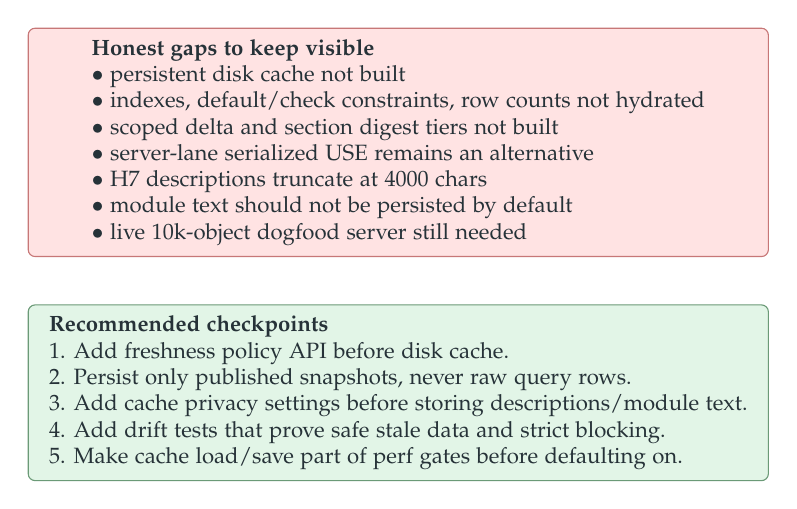
\begin{tikzpicture}[node distance=5mm]
\node[riskbox,minimum width=94mm,align=left,font=\footnotesize] (gaps) {\textbf{Honest gaps to keep visible}\\
$\bullet$ persistent disk cache not built\\
$\bullet$ indexes, default/check constraints, row counts not hydrated\\
$\bullet$ scoped delta and section digest tiers not built\\
$\bullet$ server-lane serialized USE remains an alternative\\
$\bullet$ H7 descriptions truncate at 4000 chars\\
$\bullet$ module text should not be persisted by default\\
$\bullet$ live 10k-object dogfood server still needed};
\node[goodbox,minimum width=94mm,below=6mm of gaps,align=left,font=\footnotesize] (next) {\textbf{Recommended checkpoints}\\
1. Add freshness policy API before disk cache.\\
2. Persist only published snapshots, never raw query rows.\\
3. Add cache privacy settings before storing descriptions/module text.\\
4. Add drift tests that prove safe stale data and strict blocking.\\
5. Make cache load/save part of perf gates before defaulting on.};
\end{tikzpicture}
\end{minipage}

\vspace{6mm}

\begin{tikzpicture}[node distance=8mm and 8mm]
\node[pill] (a) {Review invariants};
\node[pill,right=of a] (b) {Freeze freshness policies};
\node[pill,right=of b] (c) {Build cache codec};
\node[pill,right=of c] (d) {Wire safe consumers};
\node[pill,right=of d] (e) {Wire strict consumers};
\node[pill,right=of e] (f) {Dogfood scale};
\draw[arrow] (a) -- (b);\draw[arrow] (b) -- (c);\draw[arrow] (c) -- (d);\draw[arrow] (d) -- (e);\draw[arrow] (e) -- (f);
\end{tikzpicture}

\end{document}
